\documentclass[12pt,oneside]{article}
\usepackage{light}
\usepackage{multicol}
\usepackage{pifont} % for the star
\usepackage{palatino}
\usepackage{mathpazo}
\usepackage{verbatim}

\newcommand{\mfigure}[3]{\bigskip\centerline{\resizebox{#1}{#2}{\includegraphics{#3}}}\bigskip}
\newcommand{\hint}[1]{({\it Hint: #1})}
\newcommand{\brule}[1]{\underline{\hspace{#1}}}
\newcommand{\ang}[1]{\left< #1 \right>}
\newcommand{\beats}{\rightarrow}


\newenvironment{falseproof}
{\begin{proof}[False proof]}
{\end{proof}}

\showsolutions
%\hidesolutions

\begin{document}
\generic{Midterm}{October 27, 2010}

\instatements{
\vspace{24pt}
\textbf{Name:} \rule{5in}{0.5pt}

\textbf{Circle the name of your recitation instructor}:

\begin{center}
\begin{tabular}{llllll}
David & Darren & Martyna & Nick & Oscar & Stav 
\end{tabular}
\end{center}

\begin{itemize}

\item This quiz is \textbf{closed book}, but you may have one $8.5
\times 11$'' sheet with notes in your own handwriting on both sides.

\item Calculators are not allowed.

\item You may assume all of the results presented in class.

\item Please show your work.  Partial credit cannot be given for a wrong
answer if your work isn't shown.

\item Write your solutions in the space provided.  If you
need more space, write on the back of the sheet containing the
problem.  Please keep your entire answer to a problem on that
problem's page.

\item Be neat and write legibly.  You will be graded not only on the
correctness of your answers, but also on the clarity with which you
express them.

\item If you get stuck on a problem, move on to others. The problems 
are not arranged in order of difficulty.

\item The exam ends at 9:30 PM.

\end{itemize}

\vspace{0.25in}

\begin{center}
{\large
\begin{tabular}{|c|c|c|c|}
\hline
Problem & Points & Grade & Grader \\ \hline \hline
1 & 10 & & \\ \hline
2 & 15 & & \\ \hline
3 & 20 & & \\ \hline
4 & 10 & & \\ \hline
5 & 15 & & \\ \hline
6 & 10 & & \\ \hline
7 & 20 & & \\ \hline
Total & 100 & & \\ \hline
\end{tabular}
}
\end{center}
}
\instatements{\newpage}



\begin{problem}{10}

Consider these two propositions:
$$\texttt{P: } (A \wedge B) \implies C$$
$$\texttt{Q: } (\neg C \implies \neg A) \vee (\neg C \implies \neg B)$$ 

Use the truth table below to show whether $P$ and $Q$ are equivalent, $P \implies Q$, $Q \implies P$, or none of the above.

%
\[
\begin{array}{|c|c|c|c|c|}
\hline
A & B & C & (A \wedge B) \implies C & (\neg C \implies \neg A) \vee (\neg C \implies \neg B) \\ \hline
& & & & \\ \hline
& & & & \\ \hline
& & & & \\ \hline
& & & & \\ \hline
& & & & \\ \hline
& & & & \\ \hline
& & & & \\ \hline
& & & & \\ \hline
\end{array}
\]
%

%

\end{problem}

\newpage


%%%%%%%%%%%%%%%%%%%%%%%%%%%%%%%%%%%%%%%%%%%%%%%%%%%%%%%%%%%%%%%%%%%%%%%%%%%%%%%%%%%%%%%%%%%%%%%%%%%%%%%% Strong Induction
\begin{problem}{20}

Let $G_0=1$, $G_1=2$, $G_2=4$, and define
\begin{equation}\label{Pn}
G_n =  G_{n-1} +2G_{n-2} + G_{n-3}
\end{equation}
for $n \geq 3$.  Show by induction that $G_n\leq 3^n$ for all $n \geq
0$.

\solution{

The proof is by strong induction with hypothesis $P(n) := G_n\leq 3^n$.

\begin{proof}
\textbf{Base Cases}

\textbf{$n=0$:} $G_0 = 1 = 3^0$.

\textbf{$n=1$:} $G_1 = 2 < 3 = 3^1$.

\textbf{$n=2$:} $G_2 =f 4 < 9 < 3^2$.

\textbf{Inductive Step}:
Assume $n \geq 2$ and $P(k)$ for all $k$ such that $0 \leq k \leq n$.
\begin{align*}
G_{n+1}
& = G_n +2G_{n-1} + G_{n-2} & \text{by~\eqref{Pn}}\\
& \leq 3^n + (2)3^{n-1} + 3^{n-2} & \text{by induction hypothesis}\\
& = 3^{n-2} [3^2 + (2)3 + 1]\\
& = 3^{n-2} [(3 + 1)^2]\\
& = 3^{n-2} 4^2\\
& = 3^{n-2} 16\\
& < 3^{n-2} 27\\
& = 3^{n-2} 3^3\\
& = 3^{n+1}
\end{align*}
\end{proof}
}
\end{problem}


\newpage

\begin{problem}{0}
%Taken from: http://www.cut-the-knot.org/ctk/invariant.shtml

In the game of Squares and Circles, the players (you and your computer) start with a sequence of shapes: some circles and some squares. On each move a player selects two shapes. These two are replaced with a single one according to the following rule:

Identical shapes are replaced with a square. Different shapes are replaced with a circle.

At the end of the game, when only one shape remains, you are a winner if the remaining shape is a circle. Otherwise, your computer wins. 

\bparts

\ppart{0}
Prove that the game will end.

\solution{ Todo.}

\ppart{0}
Prove that you will win if the number of circles initially is odd. Hint: Use an invariant about the number of circles.
 
\solution{ Todo.}

\eparts

\end{problem}
%%%%%%%%%%%%%%%%%%%%%%%%%%%%%%%%%%%%%%%%%%%%%%%%%%%%%%%%%%%%%%%%%%%%%%%%%%%%%%%%%%%%%%%%%%%%%%%%%%%%%%%%%%%%%%%%%%%%%
%%%%%%%%%%%%%%%%%%%%%%%%%%%%%%%%%%%%%%%                 Martyna: number theory probs
%%%%%%%%%%%%%%%%%%%%%%%%%%%%%%%%%%%%%%%%%%%%%%%%%%%%%%%%%%%%%%%%%%%%%%%%%%%%%%%%%%%%%%%%%%%%%%%%%%%%%%%%%%%%%%%%%%%%%

\newcommand{\card}[1]{\left|#1\right|}

%number theory

\newpage

\begin{problem}{15}
\bparts
\ppart{8}
Find a number $x \in \{0, 1, \ldots, 112\}$ such that $18x \equiv 1 \pmod{113}$.

\solution{

We can do this using the pulverizer.  Specifically, if we find a pair $(s, t)$ such that $18s + 113t = 1$, then we know that $18s \equiv 1 \pmod{113}$.
\[
\begin{array}{ccccrcl}
x & \quad & y & \quad & \rem(x,y) & = & x - q \cdot y \\ \hline
113 && 18 && 5  & = &   113 - 6 \cdot 18 \\
18 && 5 && 3   & = &   18 - 3 \cdot 5 \\
&&&&            & = &   18 - 3 \cdot (113 - 6 \cdot 18) \\
&&&&            & = &   -1 \cdot 113 + 19 \cdot 18 \\
5 && 3  && 2   & = &   5 - 3 \\
&&&&						& = & (113 - 6 \cdot 18) - (-1 \cdot 113 + 19 \cdot 18) \\
&&&&            & = &   (2 \cdot 113 - 25 \cdot 18) \\
3 && 2 && 1 & = & 3 - 2 \\
&&&&            & = & (-1 \cdot 113 + 19 \cdot 18 ) - (2 \cdot 113 - 25 \cdot 18) \\
&&&&            & = &   \fbox{$-3 \cdot 113 + 44 \cdot 18$} \\
\end{array}
\]
So the multiplicative inverse of $18$ modulo $113$ is $44$.
}

\ppart{7}
Find a number $y \in \{0, 1, \ldots, 112\}$ such that $18^{112111} \equiv y \pmod{113}$
\hint{What power of $18$ is $x$ equivalent to modulo $113$?}
\solution{By Fermat's Theorem, since $113$ is prime and $113$ and $18$ are relatively prime, it must be that
\[18\cdot 18^{111} \equiv 18^{113-1} \equiv 1 \pmod {113},\]
so $x \equiv 111 \pmod {113}$.
As a result,
\[18^{112111} \equiv 18^{112\cdot 1000 + 111} \equiv {18^{112}}^1000 \cdot 18^{111} \equiv 1^{1000} \cdot x \equiv x \equiv 44 \pmod {113},\]
so the answer is $44$.
}

\eparts
\end{problem}

\newpage

\begin{problem}{10}
Define a number
$S_p = 1^p + 2^p +3^p + \ldots (p-1)^p.$
You will show in this problem that if $p$ is an odd prime, then $p|S_p$.
\bparts
\ppart{5}
 Use Fermat's Theorem to show that $S_p \equiv 1+2+\ldots + (p-1) \pmod p$.
 \solution
 {
 \begin{eqnarray*}
 S_p &\equiv& 1^p + 2^p + \ldots (p-1)^p\\
 & \equiv& 1\cdot1^{p-1} + 2\cdot2^{p-1} + \ldots + (p-1)\cdot (p-1)^{p-1}\\
 & \equiv& 1\cdot 1 + 2 \cdot 1 + \ldots + (p-1) \cdot 1\\
 & \equiv & 1 + 2 + \ldots + (p-1) \pmod p
 \end{eqnarray*}
 }
 \ppart{5}
 Show that $p|(1+2+\ldots + (p-1))$ and explain why this implies that $p$ divides $S_p$.
 \solution{
 $1+2+\ldots + (p-1) = \frac{(p-1)p}2.$\\
 $p$ is odd, so $p-1$ is even, which means $\frac{p-1}2$ is some integer $k$. Therefore
 \[1+2+\ldots + (p-1) = kp,\]
 so $p|(1+2+\ldots + (p-1))$. As a consequence, $1+2+\ldots + (p-1) \equiv 0 \pmod p$. Therefore
 \[S_p \equiv 1+2+\ldots + (p-1) \equiv 0 \pmod p,\]
 so $p|S_p$.
 }
 \eparts
 \end{problem}


\newpage

\begin{problem}[20]

Consider the simple graph $G$ given in figure $X$.

\begin{figure}[h]
\caption{Simple graph G}
\begin{center}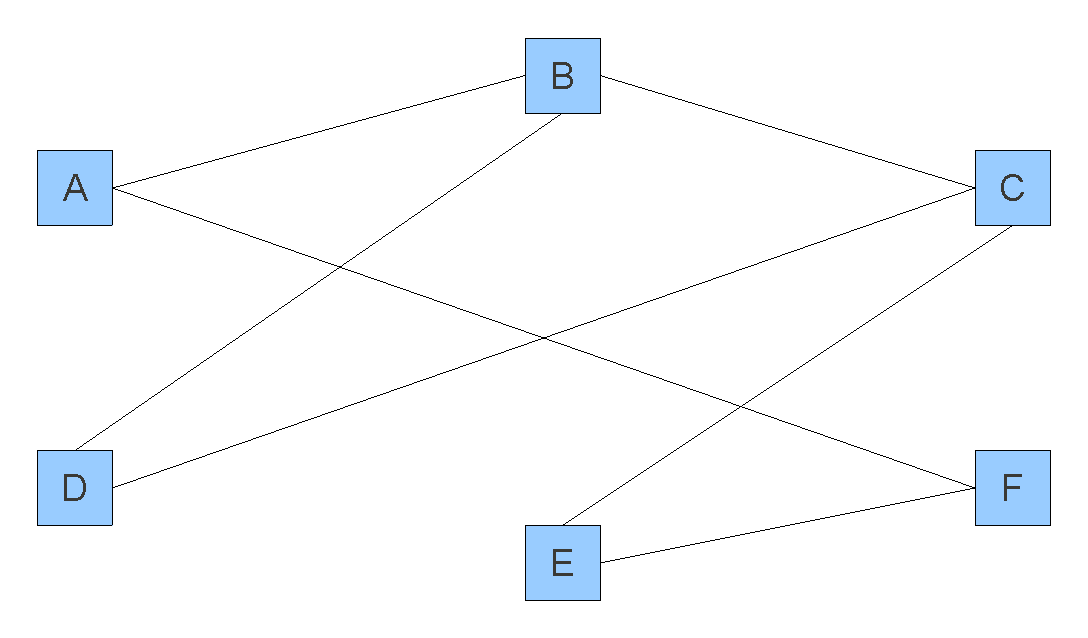
\includegraphics[width=12cm]{unweightedGraph.pdf}\end{center}
\end{figure}

\bparts

\ppart{0}
Give the diameter of $G$.

\ppart{0}
Give a longest path on $G$.

\ppart{0}
Give a coloring on $G$ and show that it uses the smallest possible number of colors.

\ppart{0}
Does $G$ have an Eulerian cycle?  Justify your answer.

\eparts

Now consider graph $H$, which is like $G$ but with weighted edges, in figure $Y$:

\begin{figure}[h]
\caption{Weighted graph H}
\begin{center}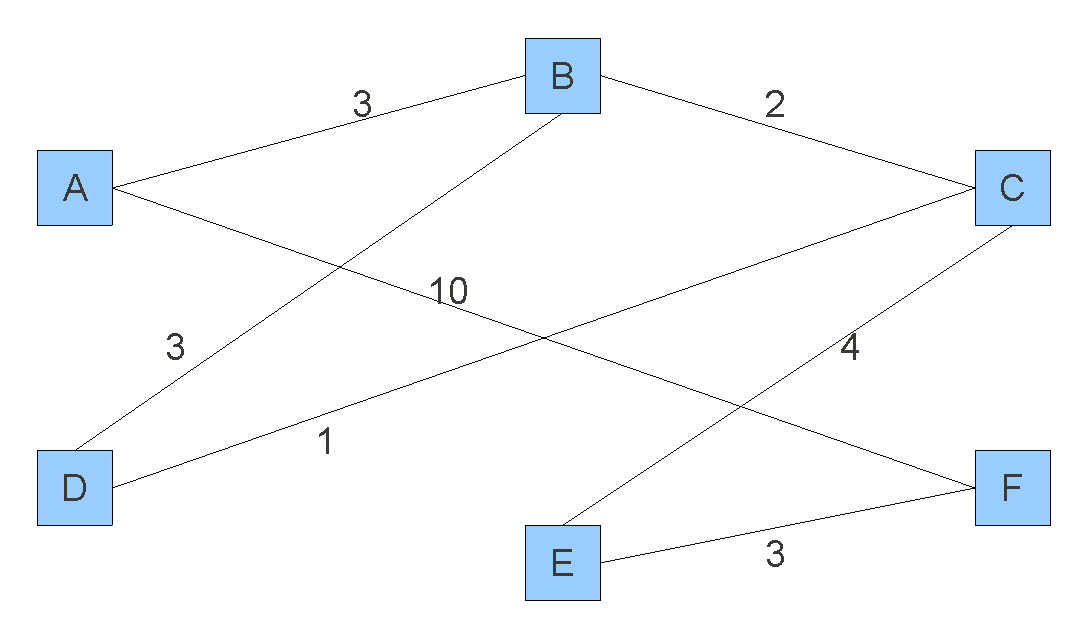
\includegraphics[width=12cm]{weightedGraph.pdf}\end{center}
\end{figure}

\bparts

\ppart{0}
Draw a minimum spanning tree on $H$.

\ppart{0}
Give a list of edges reflecting the order in which a greedy algorithm would choose edges when finding an MST on $H$.

\eparts
\end{problem}

\newpage

%%%%%%%%%%%%%%%%%%%%%%%%%%%%%%%%%%%%%%%%%%%%%%%%%%%%%%%%%%%%%%%%%%%%%%%%%%%%%%%%%%%%%%%%%%%%%%%%%%%%%%% directed graph problem. (Oscar)
\begin{problem}{20}
Consider a strongly connected directed graph with $\mathrm{indegree}(v) = \mathrm{outdegree}(v)$ for all $v \in V$. We will prove such a graph has a (directed) Eulerean tour, by considering its longest path.

\ppart {10} Show the longest sequence of adjacent edges (walk or tour) where no edges are repeated is a tour.

\solution{Consider the longest walk or tour in the graph (whichever is longer). We want to show it is indeed a tour. By way of contradiction, suppose not. Then we have a walk where each edge is different and the starting node $v_s$ is different from the end node. The starting node may have appeared in the walk on several occasions but not at the end. We can count the number of edges used on each occasion. There is the initial start edge.  From then on the rest of the edges are paired: one in for each one out of $v_s$. Hence we used up one more outgoing edge than we used incoming edges. Hence we can extend the path backwards by prefixing that missing incoming edge to $v_s$, which contradicts our walk was as long as possible.}

\ppart {10} Show no directed edge is left out of the longest possible walk or tour. 
\solution{Suppose some edge $(u,w)$ is left out from the longest path. Since the graph is strongly connected, there is a shortest path from $u$  to some $v$ in the longest tour. We can then construct an even longer path: $u,w, \cdots  v, \cdots, v$ Where we prefix the path onto the existing cycle.}

\end{problem}

%%%%%%%%%%%%%%%%%%%%%%%%%%%%%%%%%%%%%%%%%%%%%%%%%%%%%%%%%%%%%%%%%%%%%%%%%%%%%%%%%%%%%%%%%%%%%%%%%%%%%%%%%%%%%%%% graph induction on edges
\newpage

\begin{problem}{10}
Let G be a graph with $n$ vertices, $m$ edges and $k$ components. Prove that $G$ contains at least $n+ m - k  = c$ cycles. (Hint: Prove this by induction on the number of edges, $m$)

\solution{
STAV TO DO
}
\end{problem}

\newpage
%based on Fall 02, but changed
\begin{problem}{20}
The $6.042$ professors are planning to have a midterm exam and want the midterm grades to be recognized by the EECS department. This requires the completion of a number
tasks, each of which takes one hour to complete.  The prerequisites associated with these tasks are
listed below.
\begin{center}
\begin{tabular}{cll}
\textsc{Abbrv.} & \textsc{Task} & \textsc{Prerequisites} \\
S & Hold an ice cream study session & I\\
W & Write midterm questions &  I (for the TAs)\\
G & Grade the midterms & H, W\\
H & Hold the midterm & W,R,S \\
I & Buy ice cream &  \\
R & Release a sample midterm & 
\end{tabular}
\end{center}

\bparts

\ppart{4} Draw the Hasse diagram for the tasks and their
prerequisites.
  
\solution{
\begin{center}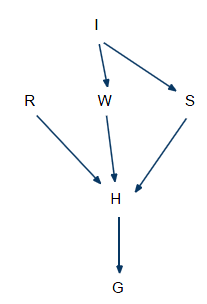
\includegraphics{hasse_diagram.png}\end{center}
}

\ppart{2} Give one ordering of the tasks that will fulfill the department's prerequisites.
\solution{
I R W S H G
}

\ppart{2} The professors have decided that since their TAs are quite
smart and they have so many of them, they can get as many tasks done at a time as
they wish.  What is the minimum amount of time required for them to
finish all the tasks? Give a sample scheduling, listing the tasks performed in each time slot.

\solution{The minimum required time is 4 (length of the critical path
I-W-H-G) A possible scheduling is:
\begin{enumerate}
\item R, I
\item W, S
\item H
\item G
\end{enumerate}
}

\eparts

Assume now that you are given a Hasse diagram with $n$ vertices in which the longest antichain has length $t$. Without knowing anything else about the graph...

\bparts
\ppart{4} ...write a simple formula in $n$ and $t$ for the maximum possible length of the longest chain in such a graph.

\solution{ In the worst case there could be a chain of size $n-t+1$ but no larger.}


\ppart{3} ...write a simple formula in $n$ and $t$ for the minimum possible length of the longest chain in such a graph.

\solution{$\ceil{n/t}$.  Since there is no antichain of size $t+1$, we know
that at least one chain must have $\geq n/t$ elements.}
\eparts
\end{problem}

\newpage




%%%%%%%%%%%%%%%%%%%%%%%%%%%%%%%%%%%%%%%%%%%%%%%%%%%%%%%%%%%%%%%%%%%%%%%%%%%%%%%%%%%%%%%
%%%%%%%%%%%%%%%%%%%%%%%%%%                 problems from Stav
%%%%%%%%%%%%%%%%%%%%%%%%%%%%%%%%%%%%%%%%%%%%%%%%%%%%%%%%%%%%%%%%%%%%%%%%%%%%%%%%%%%%%%%

\begin{problem}{0}
Induction: Prove that a sum of consecutive odd numbers (beginning with $1$); i.e. $$\sum_{i=0}^{n}2i+1$$ with $n \ge 1$; is a perfect square.

\emph{Hint: prove something stronger}
\end{problem}





\newpage


\begin{problem}{10}
Use integration to find upper and lower bounds that differ by at most
0.5 for the following sum.  (You may need to add the first few terms
explicitly and then use integrals to bound the sum of the remaining
terms.)
%
\[
\sum_{i=1}^{\infty} \frac{1}{i^3}
\]

\end{problem}


\newpage

%%O notation problem (Oscar) %%%%%%
\begin{problem}
Give a proof of the following propositions.

\begin{enumerate}
\item $x$ is $O\left( x\ln{x} \right)$
\item $x/ \ln{x}$  is $o  \left( x \right)$
\item $x^{n+1}$ is $\Omega \left( x^n \right)$
\item $n!$ is $\omega \left( n^n \right)$
\end{enumerate}

\end{problem}

\end{document}
